\section{Workflow}
Figure \ref{fig:workflow} shows the general workflow of our approach towards Boolean Function Synthesis.
1. Get the continuous equivalent of boolean specification, 2. Perform Sampling over input and output variables to obtain the trainig data,
3. Train GCLN, and 4. Extract Boolean formula from the learnt Network

\begin{figure*}[t]
	\centering
    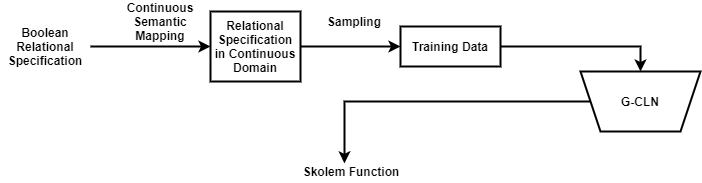
\includegraphics[scale=0.5]{workflow_bfs.png}
    \caption{Workflow}
    \label{fig:workflow}
\end{figure*}

% -------------- CODE FOR GOAL ARCHITECTURE ------------------
\subsection{Sampling Strategy}\label{sample}
Figure \ref{fig:sampling} describes the sampling pipeline that we have implemented to 
generate the training data.

\noindent\textbf{Random Sampling Strategy \Romannum{1}: }\label{sample1} In this we sample uniformly at random 
for input and output variables in the range $[0, 1]$. 
These random samples are then supplied to the continous mapping of relational specification (F). 
Output of F is then thresholded to get binary values. The ones that make F = 1 are taken to be 
positive samples. 

\noindent\textbf{Random Sampling Strategy \Romannum{2}: }\label{sample2} In this we collect positive samples 
as explained above and then add equal number of negative samples (F = 0) as well in the dataset.

\begin{figure*}
	\centering
    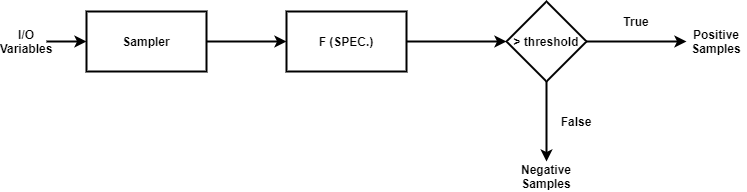
\includegraphics[scale=0.5]{sampling_bfs.png}
    \caption{Sampling Pipeline}
    \label{fig:sampling}
\end{figure*}

\noindent\textbf{Correlated Sampling: }\label{sample3} 
In this strategy, we first sample the input variables. Output variables are conditioned on input variables. 
This may help to capture the correlation betweenn input and output variables. we keep both positive and 
negative samples.

Table \ref{tab:tnorms} shows an example of random sampling.

\begin{table}[t]
\centering
\begin{tabular}{cccc}
	x: & y: & XOR(x, y) (thresholded value)\\ 
	0.9 & 0.2 & 1\\  
	0.85 & 0.01 & 1\\
    0.3 & 0.4 & 0
\end{tabular}
\caption{Example Samples for XOR(x, y) with threshold = 0.7 and Product t-norm}
\label{tab:tnorms}
\end{table}


\subsection{GCLN Architecture}\label{gcln}
Figure \ref{fig:gcln} shows the generic architecture that we use for predicting the skolem function from relational specifications.
It consists of 3 layers viz. Input Layer, Disjunction Layer, and Conjunction Layer. After each layer Gates are applied except for the final Conjunction Layer.
These Gates are the trainable weights of the neural network. More details below:

\smallskip
\noindent\textbf{Input Layer:} This layer is of shape 2N x 1, where N is the number of input variables in the given specification. 
Along with positive variables, we also consider their negations and include them in the input vector. For e.g. if the input variables 
are i1 and i2 then the input vector would contain $[i1, i2, \neg{i1}, \neg{i2}]$.

\smallskip
\noindent\textbf{Gates G1:} G1 is of shape 2N x K (K = No. of clauses and 2N = Size of each clause).
These Gates decides which input variables to be selected in each clause.

\smallskip
\noindent\textbf{Disjunction Layer:} This layer takes gated input variables. Shape of this layer is K x 1, where K is the maximum 
number of clauses that could possibly be present in the final solution. K is a hyperparameter and can be tuned.
%This layer decides which input variables to selected for each clause.

\smallskip
\noindent\textbf{Gates G2:} G2 is of shape K x 1 i.e. each node represents one of the clause. 
Here we decide upon which clause to keep as part of the solution skolem function.

\smallskip
\noindent\textbf{Conjunction Layer:} This layer takes input the gated output of the Disjunction Layer. It is of shape 1 x 1. 
%This layer decides which clauses to be selected.

\begin{figure}
	\centering
    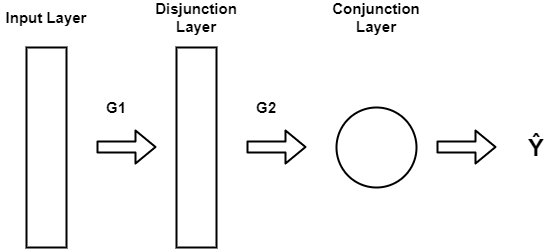
\includegraphics[scale=0.4]{gcln.png}
    \caption{GCLN Architecture}
    \label{fig:gcln}
\end{figure}

Due to the design of the network, the formula that we extract is in CNF form.
\newline

\noindent\textbf{Running Example:} Figure \ref{fig:ex} shows a running example of XOR(i1, i2, i3), 
where i1 and i2 are input variable and i3 is the output variable.

\begin{figure*}
	\centering
    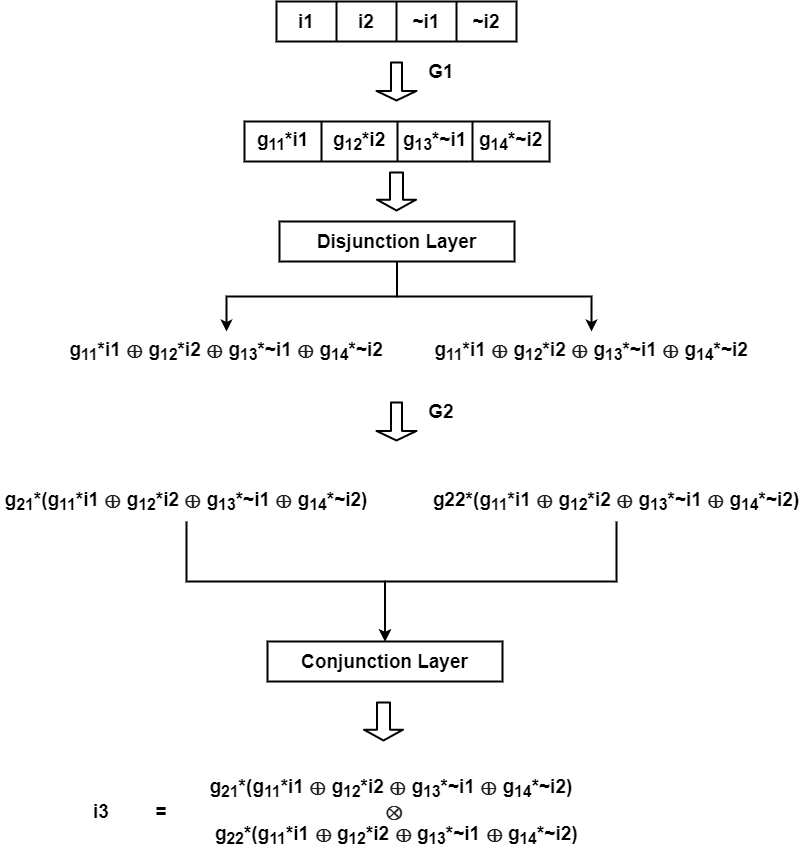
\includegraphics[scale=0.3]{example.png}
    \caption{Example run of GCLN over specification XOR(i1, i2, i3). Input Variable = i1, i2 and Output Variable = i3}
    \label{fig:ex}
\end{figure*}
% Figure \ref{fig:goal} describes the high level idea for synthesizing sketches from logical embeddings. We first sample a finite set of I/O examples from the logical specification. We wish to have a pre trained neural network for a given DSL that is trained to generate the required sketches when a logical specification and I/O specification are given as input. As a novel extension, it may also be possible for the NN to take as input a bad sketch and make decisions accordingly. This would be something similar to CEGIS(T) but using an NN. We then feed it to a traditional solver that solves the sketch using enumerative techniques if the sketch has non constant holes and constraint based techniques, if the sketch has constant holes. If the sketch is infeasible, then we use this to direct our NN to synthesize a better sketch. The meaning of an infeasible sketch is that there does not exist a valid (w.r.t. the DSL) completion of the sketch for the given specification.

% The major research question here is how to make the NN understand whether a given sketch is an infeasible sketch or not.